\chapter{Discussion}
\label{chap:discussion}

% ============ GUIDELINE AUDIT 2026-07-25 -- DISCUSSION ============
% Feeds the 15% "Testing, evaluation, critical analysis & conclusions" criterion, whose 70+ band
% reads: "Work of exceptional quality, demonstrating a clear link with ALL chapters in keeping with
% research questions/objectives. Evidence of critical and well supported analysis.
% Limitations/future research areas clearly defined."
% Full audit: docs/TCD_Dissertation/GUIDELINE_COMPLIANCE.md
%
% This is the strongest chapter in the dissertation against its criterion and needs the least work.
% It answers every hypothesis explicitly, it names three objections to its own central claim and
% answers each, it reports the fifth hypothesis as unsupported rather than rescuing it, and
% Section~\ref{sec:privacy-preserving-ai} bounds the privacy claim instead of overstating it. All of
% that is squarely 70+ behaviour and none of it should be softened.
%
% Three items only:
%
% (1) [testing 15%] LIMITATIONS vs CHALLENGES ARE NOT THE SAME THING, and only one of them is here.
%     Section~\ref{sec:limitations} covers limitations -- what the work cannot claim. The Report
%     Guidelines separately require that "any problems encountered in the course of the project
%     should be mentioned", and the marking sheet gives the examiner a CHALLENGES box asking "what
%     were the major difficulties encountered (technical or other)? Comment on the appropriateness
%     of the solutions, if any, offered." Nothing in the dissertation currently answers that box.
%     ACTION: this is addressed by adding a Challenges section to the Conclusion -- see the audit
%     header in conclusion.tex. No change needed here; the two sections should cross-reference.
%
% (2) [testing 15%] The limitations correctly concede that the judge's human agreement is unmeasured
%     and that item counts are modest -- but both concessions are qualitative. Once the bootstrap
%     intervals and the exposure-ablation results recommended in the methodology audit header exist,
%     Section~\ref{subsec:evaluation-limitations} should quote the numbers rather than the worry.
%     A limitation stated with a number is critical analysis; the same limitation stated in words is
%     a hedge, and reads to an examiner as the weaker of the two.
%
% (3) [presentation 10%] One live contraction in this chapter, fixed inline at
%     Section~\ref{subsec:transferable-framework}.
% ==================================================================

What do these results mean for the question the dissertation set out to answer? This chapter interprets the findings of Chapter~\ref{chap:experiments-results} against the five hypotheses in turn, treating the on-device assistant of Figure~\ref{fig:architecture} not as a finished product but as a probe into where trustworthy behaviour can, and cannot, be trained into a model of this size. The pattern across the five answers is read as carefully as any single one of them.

This chapter interprets the results of Chapter~\ref{chap:experiments-results} against the five hypotheses introduced.

\section{Answering the Hypotheses}
\label{sec:answering-hypotheses}

\subsection{First Hypothesis: Does Constitutional Distillation Improve Compliance?}
\label{subsec:h1-constitutional-distillation}

The first hypothesis asks the most basic question of the whole project: does \emph{constitutional distillation} actually make the model behave any better? The answer is a qualified yes. The study observed this in two parts: the first one is that the gain comes from the content of the training data and not from the act of fine-tuning itself, because format-only training actually pushed the model backwards on every single suite (Section~\ref{subsec:mr-exp1-results}), and the jump from the template condition up to the constitutional condition turns out to be the biggest single effect anywhere in the study (Table~\ref{tab:rank-lineage}). The second one is that this improvement did not land evenly across the principles: it piled up in some families like robustness, honesty and tool-discipline, and it slipped backwards in others, most clearly in the principles that ask the model to reason step by step, whose tier-level rule score actually dropped even against the untouched base (Table~\ref{tab:experiment-ladder}). 

Kyrychenko et al.\ found in the C3AI study that fine-tuning makes a model noticeably better at obeying the prohibitions than at actually performing the instructions \cite{kyrychenko2025c3aicraftingevaluatingconstitutions}, and the intuition behind that is an everyday one, since it is easier to train someone to hold back from doing a thing than to make them reliably carry a thing out. The results here fall along exactly that same line: the negatively framed robustness family improved the most while the generative reasoning principles lagged behind, so the unevenness measured here is the predicted unevenness, and not a defect in the method.

\subsection{Second Hypothesis: Does the Compliance Gain Cost Reasoning Capacity?}
\label{subsec:h2-capacity-cost}

The second hypothesis asked whether the compliance gained under the first hypothesis was bought at a price, and the study confirms that it was. The model is built to ``think out loud'' before it answers: it writes its working in a marked region called the \texttt{<think>} block and only then gives its reply, a simple analogy to a student jotting rough working in the margin before writing the final line. The visible working shows the reasoning which can be scrutinised. What the hypothesis found is that the same training that made the model more compliant also made that visible working shrink dramatically and, in most answers, disappear altogether (Table~\ref{tab:experiment-diagnostics}, Figure~\ref{fig:think-distribution}). The constitution was learned; however, the reasoning was displaced.


\subsection{Third Hypothesis: Does Prompt Engineering with Tools Match Constitutional Fine-Tuning?}
\label{subsec:h3-prompt-engineering}

The third hypothesis asks whether prompt engineering alone, with access to tools, can match a model with the constitution encoded into its weights. This is the comparison the tool-equipped baseline exists for, and it is why the vanilla conditions run under the same suites, the same student prompt and the same tool registry as the fine-tuned models. The verdict depends on the measurement lens, and the disagreement between the lenses is itself informative. Under the absolute lens, the constitutional model stays ahead of the tool-equipped baseline on the headline combined score (Table~\ref{tab:experiment-ladder}), which supports the hypothesis: instructions and grounding do not, on their own, reach what training reaches. Under the blind comparative lens, however, the two finish at overall parity (Table~\ref{tab:rank-overall}), and they win in different places: the tool-equipped baseline leads on the trust-critical outcome principles, where real grounding beats trained behaviour whenever a fact is demanded, while the constitutional model leads on the reasoning and personalisation substrate and on tool discipline (Table~\ref{tab:rank-tiers}). The honest reading is that prompt engineering with tools goes further than the hypothesis expected, but it does not replace training: the two mechanisms buy different layers of trustworthy behaviour, and that layered result is more useful than a single winner would have been.

\subsection{Fourth Hypothesis: Where Are the Failure Boundaries? (Is the Boundary Systematic?)}
\label{subsec:h4-failure-boundaries}

The fourth hypothesis turns a negative result into a usable finding. The question was not \emph{whether} the fine-tuned model fails, but whether its failures are \emph{systematic}, that is, predictable in advance from the kind of task and the way the prompt is phrased, rather than scattered at random. The finding is that they are systematic. The principles that stay out of reach are reliably the same ones, those that demand genuine multi-step reasoning, such as working a problem from first principles or gathering context through the 5W+H questions, and they tend to fail together and in the same direction even as the wording of the prompt is varied (Figure~\ref{fig:rank-principle-heatmap}). 

This boundary echoes two failure modes already documented in larger systems. Potham reports an ``illusion of compliance'', in which a cautious model scores well by doing very little \cite{potham2025evaluatingllmagentadherence}, and Liu et al.\ observe a drift towards merely doing what the user asks whenever a model is handed conflicting instructions \cite{liu2026generativevalueconflictsreveal}. The brittleness of very small models, their habit of breaking on a lightly reworded problem, has likewise been reported by Rainone et al.\ and by Wei et al., the former tying it to the interaction of small scale with free-form chain-of-thought reasoning rather than to scale alone \cite{rainone2025replacingthinkingtoolusage, wei2025reactplannercentricframeworkcomplex}. What this work adds is to locate that boundary specifically at the 0.6B scale and to ask what causes it.

On the question of cause, the evidence leans towards scale rather than data, though it does not point that way unanimously, and saying so plainly is part of the result. Experiment~2 fed the model a larger and much higher-quality constitutional dataset and yet the reasoning still did not come back, which is exactly what one would expect if the real limit were genuinely one of capacity and not one of examples. And yet a single model, trained and tested on its own, cannot completely rule out that some subtler property of the data is to blame. That leftover doubt is less a loose end than a motivation, because it is why Experiment~3 splits the task across two models, to see whether relieving the capacity pressure, rather than improving the data, is what moves the boundary.

The per-principle heatmap is the visual form of the hypothesis claim (Figure~\ref{fig:rank-principle-heatmap}), because if the failure boundary were random its cells would look like noise, and instead every condition shows these coherent blocks of strength and weakness that line up with whatever its training actually contained. 


% [STYLE 2026-07-24] ACTION: CONSIDER (judgement call, not mechanical): REPLACE, or append after, the thin live paragraph above starting "The per-principle heatmap is the visual form" WITH the richer five-profiles synthesis below.
% (Context: a SUBSTANTIVE alternative kept during the STYLE-block consolidation that removed the nine Introduction/Motivation-register duplicates elsewhere in this chapter; NOT a register swap but a richer five-profiles synthesis that strengthens the fourth-hypothesis close. Swap in / merge if approved.)
% Read together with the finishing-position and grade profiles (Figures~\ref{fig:rank-distribution} and~\ref{fig:rank-grade-profile}) and the family fingerprints (Figure~\ref{fig:rank-model-profiles}), the five conditions resolve into five distinct behavioural profiles rather than five points on a single line. The untrained base model is the mid-fielder: without tools it can neither ground nor verify, so it hedges and occasionally fabricates, and it is rarely the best and rarely the worst. The tool-equipped baseline is the consistent professional: it grounds what it can and declines what it cannot, and its grades sit in the middle-upper band with few catastrophes, which is why it wins the direct duels it might be expected to lose (Figure~\ref{fig:rank-pairwise-matrix}). The template model is the cautionary case: trained on format without content, it reasons privately and returns empty or broken answers, with right-direction-but-failed-execution as its most common grade. The constitutional model is the polarised specialist: its grades concentrate at both ends, ideal where the constitution trained a behaviour and fabricating fluently where a fact was demanded that its weights could not supply. The dual model is the peak-only clarifier: the only condition that asks before assuming, ideal on the ask-shaped questions and unreliable where the hand-off forces it to improvise. Stated in one sentence, the boundary between these five profiles follows the training data of each condition, not the difficulty of the questions, which is what the fourth hypothesis predicted.

\subsection{Fifth Hypothesis: Does Two-Model Decomposition Move the Single-Model Ceiling, On-Device?}
\label{subsec:h5-thinker-executor}

The hypothesis here was that separating the thinking from the execution would give each 0.6B model an undivided parameter budget and its attention over just a single-role context, and that the two specialised models working together would recover capability that a single 0.6B model simply cannot reach on its own. The comparative lens then forces a certain honesty about that claim which has to be stated plainly, that the hypothesis was formulated on the expectation that the single constitutional model would turn out to be capacity-bound, and the dual architecture was built as the structural escape from exactly that bound. The head-to-head results then partly overturn that premise. Ranked blind, the single constitutional model is the strongest of the five conditions on the weighted score, and the dual model trails behind it on the weighted score (Figure~\ref{fig:rank-lineage}); so under this lens the final stage of the whole progression subtracts rather than adds.

A fair reading of Experiment~3 has to begin with where the dual model's data comes from. The Thinker and the Executor are not trained on a separate corpus: the trajectory splitter (Section~\ref{subsec:mr-dataset}) projects the same constitutional trajectories that train the single model onto two role-conditioned views, so the comparison isolates the architecture rather than the data. That makes the dual model's weaker headline result harder to dismiss, and also easier to locate. Because the two views are read from one trajectory, the Thinker inherits exactly the reasoning the corpus contains and no more. Where the single model can lean on answer formatting and on tool use to mask a thin reasoning trace, the Thinker has only the trace: its entire job is the one signal the corpus was least able to supply, given the capture-fidelity ceiling of the trajectories it shares with every other condition. The architecture therefore does not fail in principle; it is maximally exposed to a limitation of the synthetic data it shares with every other condition, so the mechanism the hypothesis names never got a fully clean test. Experiment~3 is read as architecture under data constraint, not architecture refuted.

Two causes of the deficit are separable. The first is the data inheritance just argued, to which the judge's per-answer evidence adds a failure mode the absolute scores had folded into one number: fabricated tool calls and results appearing in the trace around the hand-off. The second is architectural: the orchestration adds a hand-off on every turn, and a single malformed plan breaks the chain, which is exactly where the long-conversation drift suite records the study's weakest cell (Table~\ref{tab:experiment-ladder}). On-device, a deployment must additionally either hold both checkpoints resident or pay a reload at each hand-off, so at the observed deficit the single constitutional model is the more deployable artefact on most axes measured.

That same lens also gives the dual model its honest credit, and the two worked case studies reported back in the results chapter (Tables~\ref{tab:case-p5} and~\ref{tab:case-p6}) carry the whole argument in miniature. On the real-time honesty case the constitutional model is graded ideal while the dual model fabricates a market cap, a price and a date after its tool calls fail; on the context-gate case the roles invert almost exactly, with the dual model asking the one targeted question the constitution actually wants asked while the constitutional model invents a whole list of plausible-sounding book titles. The dual model stays the only condition that clarifies at all, its wins concentrate on the highest-weight questions, and it shares the best purpose-weighted win share with the constitutional model even while its headline average trails (Table~\ref{tab:rank-overall}). Peak behaviour and consistency have therefore come apart here: the dual architecture is ideal precisely where its role split points it, and unreliable almost everywhere it is forced to improvise. The fifth hypothesis is therefore left as unsupported on its headline claim at the present data quality, with its distinctive strengths named, and with the two named confounds, the data inheritance and the hand-off cost, marking out exactly what future work would have to change before the question is even worth re-asking. The stronger counterfactual, that the same split would lead at a higher trace fidelity, is not claimed here because it is untested; it is stated instead as a concrete prediction that future work can falsify, with the remedy set out as reasoning-preserving self-distillation in Section~\ref{subsec:conclusion-future-data}.

\section{The Alignment Tax at the 0.6B Scale}
\label{sec:capacity-displacement-trade-off}

The idea that connects the preceding hypotheses is a single one: at 0.6 billion parameters, the model's representational \emph{capacity}, loosely, the total amount of skill its adjustable numbers can encode, behaves like a fixed budget that several demands draw on at once. Reasoning draws on it, reliable tool use draws on it, and obeying the constitution draws on it. The consequence is that training does not enlarge this budget; it redistributes it. Fine-tuning a small model, then, is better understood not as \emph{addition} but as \emph{reallocation}: a behaviour gained has, in general, been paid for by a behaviour given up somewhere else (Figure~\ref{fig:displacement-concept}). Read this way, the uneven improvement found under the first hypothesis and the lost reasoning found under the second stop being two separate observations and become one phenomenon seen from two angles, the form taken at this scale by what the literature calls the \emph{alignment tax} \cite{askell2021generallanguageassistantlaboratory, ouyang2022traininglanguagemodelsfollow} and, in its reasoning-specific guise, the \emph{safety tax} \cite{huang2025safetytaxsafetyalignment, fu2026reducingsafetytaxllm}.

\begin{figure}[H]
  \centering
  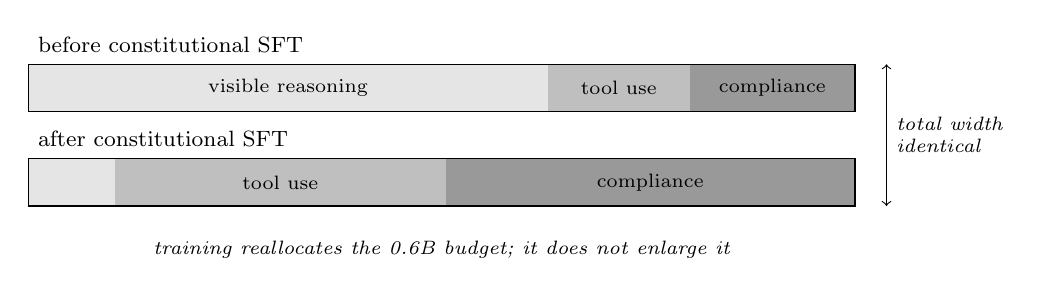
\begin{tikzpicture}[font=\scriptsize]
    % before SFT
    \node[anchor=west, font=\footnotesize] at (0,2.05) {before constitutional SFT};
    \fill[black!10] (0,1.2) rectangle (6.6,1.8);
    \fill[black!25] (6.6,1.2) rectangle (8.4,1.8);
    \fill[black!40] (8.4,1.2) rectangle (10.5,1.8);
    \draw (0,1.2) rectangle (10.5,1.8);
    \node at (3.3,1.5) {visible reasoning};
    \node at (7.5,1.5) {tool use};
    \node at (9.45,1.5) {compliance};
    % after SFT
    \node[anchor=west, font=\footnotesize] at (0,0.85) {after constitutional SFT};
    \fill[black!10] (0,0.0) rectangle (1.1,0.6);
    \fill[black!25] (1.1,0.0) rectangle (5.3,0.6);
    \fill[black!40] (5.3,0.0) rectangle (10.5,0.6);
    \draw (0,0.0) rectangle (10.5,0.6);
    \node at (3.2,0.3) {tool use};
    \node at (7.9,0.3) {compliance};
    % annotations
    \draw[<->] (10.9,0.0) -- node[right, align=left, font=\scriptsize\itshape]{total width\\identical} (10.9,1.8);
    \node[align=center, font=\scriptsize\itshape] at (5.25,-0.55)
      {training reallocates the 0.6B budget; it does not enlarge it};
  \end{tikzpicture}
  \caption{The alignment tax as a fixed budget: constitutional fine-tuning reallocates a 0.6B model's capacity towards compliance and tool use at the expense of visible reasoning, rather than adding capability.}
  \label{fig:displacement-concept}
\end{figure}

The reason for confidence that this is genuine reallocation rather than a measurement artefact is the precise shape of what was observed: the gain and the loss are yoked together. At the point where compliance and tool discipline climb, the visible reasoning trace collapses (Section~\ref{subsec:mr-exp2-results}, Table~\ref{tab:experiment-diagnostics}). A bad run, a flaky test, or noise would tend to push every measure down together or vary the numbers at random; a clean something-up, something-down trade is instead the fingerprint of a single shared resource being fought over. That Rainone et al.\ report a comparable brittleness in other small models is consistent with reading capacity as the binding constraint here, although their further demonstration that a more structured reasoning format partly recovers it is a reminder that the constraint is not scale alone \cite{rainone2025replacingthinkingtoolusage}.

A claim this central should be made to survive its obvious objections, so three are named and each answered. The first is that this is merely a \emph{data} artefact, too few or too poor training examples; Experiment~2 answers it in part by supplying a larger, cleaner constitutional dataset and finding that the reasoning still does not come back, though the under-capture of that corpus's reasoning traces means the data explanation is reduced rather than eliminated. The second is a \emph{decoding} artefact, the worry that the model is only seen producing shorter text because of one setting of its sampling ``temperature''; every condition was decoded under identical settings, so a decoding artefact would have to suppress the fine-tuned model's reasoning while leaving the base model's intact under the same configuration, which is implausible, though a full temperature sweep would settle the point. The third is a \emph{probe} artefact, the worry that the measure simply rewards verbosity; the structural, model-free check answers it, because it asks only whether a non-empty reasoning block is present at all, never how long or how eloquent it is. With those three addressed, displacement is the reading left standing, and it is precisely why the structural move of this dissertation, dividing the budget across two specialised models, is a designed response rather than incidental engineering.

Framing the remedy through the budget account is also what makes it testable, because it predicts not a vague improvement but a \emph{sharp, directional} one: help should appear precisely where the single model was starved, in the visible reasoning that collapsed under fine-tuning, and not as a uniform lift everywhere. Experiment~3 lands exactly there (Section~\ref{subsec:h5-thinker-executor}): the empty-trace rate falls, the trace lengthens, and the ask-before-assuming behaviour emerges only in the split, while nothing else rises uniformly. That the gain fell in the reasoning and clarification behaviours the role split targets, rather than everywhere at once, is also what separates genuine \emph{specialisation} from merely throwing \emph{more compute} at the problem, and a result that arrives in the predicted place is more convincing than one that is merely larger. The broader question of whether several small models can club together to beat a single one has been asked before by Zywot et al.\ \cite{zywot2026smallagentscollaboratebeat}; the departure here is that both models stay on the device.

\section{Privacy-Preserving AI: Does This Architecture Deliver?}
\label{sec:privacy-preserving-ai}

On its own terms, the architecture secures a specific, bounded form of privacy by construction rather than by policy. At the moment of answering, nothing about the user's conversation leaves the device: the user-model graph that stores what the system believes about the person, and the scratchpad that carries the thread of the conversation, both live in the device's own storage, and no request carrying the user's words is ever sent to a server in the cloud. Measured against the motivation this work began from, and against what the General Data Protection Regulation asks of any system holding the most sensitive, ``special-category'' personal data \cite{gdpr2016}, this is exactly the property the whole on-device decision was meant to secure, and the system built here keeps it.

Honesty requires being exact about the limits of that guarantee, because it is narrower than the bare word ``privacy'' might suggest. There are two quite different privacies in play. One is \emph{data} privacy, about the user's own conversations, and that is the one achieved: those conversations are not transmitted. The other is \emph{training} privacy, about the enormous body of text the base model was built from long before it ever reached the device, which was scraped from the open internet and lies entirely outside anything this work can change. The first is secured; the second cannot be touched. Two further residual surfaces deserve to be named rather than buried: the local store still physically holds a profile of the person, so the security of the device itself becomes part of the trust story, and the constitution being enforced was written by the researcher, not by the user, so the values in force are the researcher's and not yet the user's. The guarantee is real and worth having; it is also bounded, and stating those bounds plainly is itself part of being trustworthy.

% ==================================================================================================
% [DRAFT 2026-07-25 | testing/evaluation/conclusions (15%)] TWO STRUCTURAL UPGRADES TO THIS CHAPTER.
% Both are about the reader connecting dots, not about adding content -- the material already exists
% and is in the wrong shape or the wrong place.
%
% ---------------------------------------------------------------------------------------------
% UPGRADE 1: PROMOTE THE LENS DISAGREEMENT FROM A SUB-POINT TO A FINDING.
%
% The most interesting thing this dissertation discovered about MEASUREMENT is that its two lenses
% disagree, and that the disagreement is systematic rather than noise: the absolute lens favours the
% fine-tuned model, the blind comparative lens ties it with the tool-equipped baseline, and the tier
% decomposition explains exactly why (grounding wins trust-critical outcomes, training wins the
% substrate). That is a genuine contribution to how small-model compliance should be evaluated.
%
% Right now it is buried as the verdict of the third hypothesis
% (Section~\ref{subsec:h3-prompt-engineering}). But the dissertation's stated primary contribution is
% "a framework for MEASURING and improving constitutional behaviour" -- so the finding that a single
% lens would have given the wrong answer IS the contribution demonstrating itself, and it is filed
% as a hypothesis result instead.
%
% ACTION: add a short section after Section~\ref{sec:capacity-displacement-trade-off}, e.g.
% \section{Why One Measurement Lens Is Not Enough}, making three points that are already established
% and merely need collecting:
%   (a) An absolute judge grading against a constitutional ideal compresses every condition towards
%       the bottom at this scale, because no 0.6B model reaches the ideal
%       (Section~\ref{subsec:mr-judge-validity}) -- so absolute scores understate the differences a
%       reader can plainly see in the transcripts.
%   (b) A comparative judge answers the reader's question but cannot say whether ANY condition is
%       good, only which is better -- a field of five weak answers still produces a winner.
%   (c) Deterministic probes cannot be charmed but under-credit correct behaviour phrased unexpectedly,
%       and the hollow-pass rate you already measure quantifies exactly how often form is rewarded
%       over substance.
% Then state the consequence plainly: the three instruments fail in DIFFERENT directions, which is
% why the study reports all three and why the third hypothesis returns a layered rather than a single
% answer. Close by noting that a study using only one lens would have reported a clean win for
% constitutional fine-tuning and been wrong.
% This also strengthens Conclusion contribution 2 (the judge-as-instrument claim), which currently
% asserts rigour that this section would demonstrate.
%
% ---------------------------------------------------------------------------------------------
% UPGRADE 2: GIVE Section~\ref{sec:limitations} THE STANDARD VALIDITY STRUCTURE.
%
% The three limitation subsections that follow are honest and well-judged, but they are organised by
% SUBJECT (model, evaluation, data). Reorganising them under the four standard validity headings costs
% almost no new writing, and buys two things: an examiner can check coverage at a glance, and the
% reader sees which threats are controlled versus merely acknowledged -- the difference between
% "limitations defined" (60-70 band) and "critical and well supported analysis" (70+).
%
% Proposed mapping of what is ALREADY written, plus the gaps it exposes:
%
%   CONSTRUCT VALIDITY -- does compliance with these principles measure trustworthiness?
%     Have: the construct-validity paragraph in Section~\ref{subsec:evaluation-limitations}; the
%     grounding of persona dimensions in Mayer et al. and Davis
%     (Section~\ref{subsec:psychological-foundations}).
%     GAP: the judge exposure ablation (full / bare / none) speaks directly to this and its results
%     are unreported -- see the methodology audit header. Reporting it converts this from a conceded
%     worry into a measured one.
%
%   INTERNAL VALIDITY -- can each difference be attributed to the factor changed?
%     Have: the staged single-factor ladder; identical decoding across conditions; the shared-corpus
%     control that isolates architecture from data in Experiment~3; the three answered objections in
%     Section~\ref{sec:capacity-displacement-trade-off}.
%     GAP: state plainly the two confounds that remain -- a single teacher model, and the
%     reasoning-capture defect that affects the Thinker most of all.
%
%   EXTERNAL VALIDITY -- how far do the results travel?
%     Have: Section~\ref{subsec:model-scale-limitations} on single-model, single-family.
%     GAP, AND IT IS A STRENGTH GOING UNCLAIMED: the question set was generated across sixteen
%     situation categories and twenty region, culture and demographic axes, with local currencies, tax
%     regimes and financial practice. That is a deliberate defence against Western-default evaluation
%     and it is currently invisible in the live text (see the [AUDIT 2026-07-24] block in
%     methodology-results.tex). It belongs here as a positive external-validity argument, and it
%     answers a question a linguistics second reader is quite likely to ask. State also the honest
%     bound: all questions and all judging are in English.
%
%   CONCLUSION VALIDITY -- are the inferences from the numbers sound?
%     GAP: this heading is currently empty and it is where the missing intervals belong. Once the
%     paired bootstrap recommended in the methodology audit header exists, this subsection states the
%     item counts, the intervals, and which observed differences survive them. Until then, the parity
%     claim of the third hypothesis rests on an unquantified appeal to noise.
%
% Keep every existing bound-and-defence pairing -- "the limitation is X, the bound on it is Y" is
% doing real work and is a large part of why this chapter reads as mature. Only the headings and the
% four gaps above change.
% ==================================================================================================
\section{Limitations}
\label{sec:limitations}

\subsection{Model and Scale Limitations}
\label{subsec:model-scale-limitations}

The most obvious limitation is that everything here rests on a single model, Qwen3-0.6B, of a single architectural family, the decoder-only transformer that underlies most of today's chat models. One cannot assume the specific numbers would survive a change of model: a differently-built small model such as Phi-3-mini, SmolLM or Gemma-2B, or a more unusual design such as an encoder-decoder or a state-space model, might sit at a different point on every measure reported. A reader is right to read the figures as pertaining to this model, not to small models in general.

The bound on that limitation is what keeps it from undermining the contribution, and it is worth stating clearly: it is the \emph{numbers} that are single-model, not the \emph{method}. The framework that produced them, the deterministic probe suites, the dual-lens judging protocol, and the staged single-factor design, was built to be model-agnostic, so the proper response to ``does this generalise?'' is not to argue about it but to re-run the framework on another model and read the answer off. That is exactly why cross-model replication is the first item of future work (Section~\ref{subsec:conclusion-future-extensions}): the single-model result is the first data point, not the whole claim.

\subsection{Evaluation Limitations}
\label{subsec:evaluation-limitations}

Three limits attach to how things were measured. The first is the deepest, and it is a measurement worry the second reader will recognise from their own field: \emph{construct validity}, that is whether the thing being scored, compliance with these written principles, is the thing being claimed, trustworthiness, or only a convenient stand-in for it. Trustworthiness has been defined as compliance with a written constitution, which is precise and checkable, but precision is not the same as completeness, and no pretence is made that the probes settle the larger question. The second is statistical: there are only so many probes in each suite, and a modest number of test items yields wide uncertainty around any single rate, which is why paired comparisons on identical questions, and the convergence of two independent lenses, are relied on rather than standalone headline numbers.

The third, and the most exposed limitation here, is that there was no human evaluation: every result in this dissertation is a statement about how the model \emph{behaves}, as measured by deterministic probes and a rubric-constrained language-model judge, not about how a person \emph{perceives} it, and the judge's agreement with human markers is itself unmeasured. The bound here is twofold. The deterministic probes deliberately trade some breadth for objectivity: they measure a narrower thing, but they measure it the same way every time and cannot be charmed, and they accompany every judge-based number as its judge-free anchor; and the missing human study is not quietly ignored but scoped explicitly as future work (Section~\ref{subsec:conclusion-future-user-studies}). Automated probes can show that the system behaves trustworthily; only users can show whether it feels that way, and care is taken not to claim the second on the strength of the first.

\subsection{Training Data Limitations}
\label{subsec:training-data-limitations}

The training set carries three related limitations. It is small; it is synthetic, generated by this work's own pipeline rather than drawn from a large independent source; and its reasoning traces were only partially captured, so on many turns the model was shown answers with the thinking already removed. Each is a genuine risk: a principle with few examples may be under-trained, any bias in the generated ``gold'' answers is copied faithfully into the student, and under-captured reasoning teaches a model to omit reasoning.

The bound is that the smallness is in part a deliberate design choice rather than only a shortfall, and this matters for how seriously it threatens the claims. On the LIMA evidence set out in the background (Section~\ref{subsec:training-data-quality-vs-quantity}), a compact, curated set is a defensible instrument rather than a weakness, and it carries an underrated virtue: its biases are \emph{traceable} rather than diffuse, because exactly what it contains is known. Because Experiment~2 substitutes a better dataset while holding the model and recipe fixed, the design separates the effect of the data from the effect of the scale in a way a single uncontrolled corpus could not.

% ==================================================================================================
% [DRAFT 2026-07-25 | testing (15%) + technical (50%)] THE EPISTEMIC STATUS OF THE "GOLD" DATA.
% GAP: the dissertation states five times that the corpus is synthetic, but nowhere states what that
% means for the strength of the claims. The word "gold" is used throughout (and once in scare quotes
% here) without ever saying that nobody verified these responses are good -- they are assumed good
% because a capable teacher produced them under the right instructions. An examiner will notice the
% assumption; far better to name it first. Naming it also lets you state what a real gold standard
% would take, which is exactly the "critical approach to analysis" the 70+ band rewards, and which
% costs nothing because the answer is a limitation you already live with.
% Place as two paragraphs immediately after the paragraph above. To apply, delete the "% " prefixes.
%
% A further point about the training data deserves to be stated directly rather than left implicit. The examples that train every fine-tuned condition are described throughout as \emph{gold} responses, but nothing in this study establishes that they are in fact ideal. They are the outputs of a frontier-scale teacher answering with the constitution in view, retained by a length-based quality gate, and they are treated as good because a capable model produced them under the right instructions, not because any person read them and agreed. That assumption is reasonable, and it is the ordinary basis of distillation, but it is an assumption and it propagates: whatever the teacher misjudged, the student learns faithfully and the probes cannot detect, because the same document that shaped the teacher also shaped the rubrics.
%
% What a genuine gold standard would require is worth naming, because the distance between it and what was used here bounds every training claim made in this dissertation. It would require examples authored or vetted by people with domain competence across the areas probed; more than one annotator per item, so that disagreement between them is visible rather than absorbed; an adjudication procedure for the items on which they disagree; a reported inter-annotator agreement statistic, so that the reliability of the resulting labels is characterised rather than assumed; and a held-out portion never seen during generation, against which the corpus itself could be validated. None of this was reachable within the time, budget and ethical-approval constraints of a single-author project spanning sixteen question categories and twenty cultural contexts, and so a teacher model stood in for the panel of annotators. The substitution is defensible and it is standard practice at this scale, but it should be read as a constraint the work operated under, not as a property of the data.
% ==================================================================================================

\section{Implications for Practice}
\label{sec:implications-practice}

The practical lesson of this work is architectural rather than numerical, and it can be put in one line: at 0.6B, trustworthiness is bought in layers, and no single layer buys all of it. Three takeaways follow. Grounding comes first: a curated system prompt with real tool access lifted the untrained model to the best trust-critical outcomes in the study, at the cost of no training at all. Training buys the substrate: constitutional distillation delivered the reasoning-adjacent, robustness and tool-discipline behaviours that instructions alone did not, but it redistributed capacity to do so, and what it displaced had to be measured with judge-free diagnostics to be seen. And some principles, the reasoning-heavy ones, stayed out of reach of every intervention tried at this scale and will likely require a larger model rather than a cleverer small one.

% [TRIM] ACTION: CONSIDER (judgement call, not mechanical): REMOVE the guidance table to save ~0.5pp -- cut Table~\ref{tab:guidance} and keep the live prose paragraph starting "Those lessons land differently", OR cut that prose paragraph and keep the table, NOT both.
% (Table~\ref{tab:guidance} (Developer/Researcher/Policy) restates this very paragraph in table form; the two say the same thing twice. Academic view: a three-row table adds no information a reviewer cannot get from the sentence.)
Those lessons land differently for the three audiences this work touches (Table~\ref{tab:guidance}), though they differ in emphasis rather than substance. A developer building an on-device assistant should give the model grounding before training, not instead of it, and should measure what any fine-tune displaces, not only what it adds. A researcher studying small-model compliance should treat it as a measurement problem with a locatable boundary, where the interesting question is not ``does it comply?'' but ``where exactly does it stop complying, and why?''. A policy reader weighing privacy-preserving AI should take away that, at this scale, keeping data on the device and achieving full constitutional compliance are not yet simultaneously free, a trade-off worth understanding before it is written into a requirement. In each case the guidance is pitched at the level of method, not numbers, because one model's exact figures should not be hardened into advice.

\begin{table}[H]
  \centering
  \caption{Practitioner guidance by audience; deliberately method-level, not number-level.}
  \label{tab:guidance}
  \begin{tabular}{lp{11.4cm}}
    \toprule
    Audience & Takeaway \\
    \midrule
    Developer & Ground before training: real tool access buys the trust-critical outcomes cheaply; fine-tuning buys the behavioural substrate but displaces capacity, so measure what training removes as well as what it adds. \\
    Researcher & Treat small-model compliance as a measurement problem with a locatable boundary: the question is not ``does it comply?'' but ``where exactly does it stop complying, and why?''. \\
    Policy & On-device privacy and full constitutional compliance are not yet simultaneously free at this scale; understand the trade-off before writing it into a requirement. \\
    \bottomrule
  \end{tabular}
\end{table}


% [AUDIT 2026-07-24 -- TRIM directive (Owen: "think what you want the reader to absolutely know, then
% define the content; be rational enough to remove content however well it reads")] ACTION: CONSIDER (judgement call, not mechanical): keep statement 1 (this subsection, the fullest statement) and statement 4 (Conclusion future work, Section~\ref{subsec:conclusion-future-extensions}) at length; shorten statement 2 (Section~\ref{subsec:model-scale-limitations}) to a one-line back-reference to here, and statement 3 (Conclusion contribution 1, Section~\ref{sec:conclusion-contributions}) to a single clause. Net saving ~0.5-0.75pp. Full rationale, the five repetition sites, the reader's-takeaway yardstick and the DONE-2026-07-24 status note follow below.
% This subsection is
% the CANONICAL home of the dissertation's single most-repeated message -- "the contribution is a
% model-agnostic framework, not a verdict on one model; re-run it on the next model". That message is
% currently stated in FIVE places that say substantially the same thing:
%   1. HERE (Section~\ref{subsec:transferable-framework}) -- the fullest statement; KEEP this one.
%   2. Section~\ref{subsec:model-scale-limitations} above ("the numbers are single-model, not the method
%      ... re-run the framework on another model ... cross-model replication is the first future work").
%   3. Conclusion contribution 1 (Section~\ref{sec:conclusion-contributions}) -- "reusable, model-agnostic
%      framework ... re-run on the next model to locate that model's boundary".
%   4. Conclusion future work (Section~\ref{subsec:conclusion-future-extensions}) -- "a framework that
%      calls itself model-agnostic has only made a claim until it is run on a second model".
%   5. (Would have been a 6th in the methodology; that draft was deliberately reduced to a MECHANISM-only
%      paragraph that cross-references here -- see Section~\ref{subsec:mr-runbook} preceding comment.)
% RECOMMENDATION: keep 1 and 4 (they do different jobs -- 1 is the interpretive claim, 4 is the concrete
% experiment). Shorten 2 to a one-line back-reference to here, and 3 to a single clause, since a
% contributions list should assert the contribution, not re-argue it. Net saving ~0.5-0.75pp and, more
% importantly, the message lands harder for being made once with force rather than four times softly.
%
% THE READER'S TAKEAWAY YARDSTICK (for judging every other candidate cut in Discussion+Conclusion):
% the four things a reader must carry away are (a) constitutional distillation works below 1B but
% (b) at a measured safety tax -- capacity is reallocated, not added; (c) grounding and training buy
% DIFFERENT layers of trust (the lens-split result); and (d) the durable contribution is the measurement
% framework, not the verdict. Content that does not serve one of these four is a cut candidate.
% DONE 2026-07-24: the nine redundant "Introduction/Motivation register" [STYLE] duplicates in this
% chapter were removed (the live analytical register is correct for a Discussion; one was also inferior,
% silently dropping the alignment-/safety-tax naming and four citations). One STYLE block remains -- the
% SUBSTANTIVE five-profiles synthesis after the fourth-hypothesis heatmap paragraph -- because it adds
% content rather than merely re-registering it.
\subsection{A Transferable Framework, Not a Verdict}
\label{subsec:transferable-framework}

It would be easy to read this dissertation as answering a yes/no question, can a small 0.6B model be made trustworthy?, and to treat the answer as its contribution. That reading does not account for the reasoning behind it. A verdict on one model expires the moment a more capable small model is released; as the space of language models is rapidly evolving and the models are frequently upgraded, the procedure used to reach the verdict does not. The durable contribution is a model-agnostic framework: a suite of deterministic constitutional probes, a dual-lens judging protocol whose design controls are stated, and a staged single-factor experimental design. Applied to Qwen3-0.6B, the framework located a specific safety-tax boundary; applied to next year's model, it would locate that model's boundary instead. The dissertation is therefore better read less as the claim ``this model can comply'' and more as the tool ``here is how to measure and improve compliance in whatever small model must be deployed on-device''.


% [DRAFT 2026-07-25 | reader retention | DEVICE A -- CHAPTER-CLOSING BRIDGE]
% Final bridge, into the Conclusion. Append as the last paragraph of the chapter. To apply, delete
% the "% " prefix.
%
% The interpretation is now complete. Compliance and visible reasoning trade against one another at this scale because capacity behaves as a fixed budget that training redistributes rather than enlarges, and trustworthy behaviour is consequently bought in layers that no single intervention supplies at once. What remains is to state plainly what the dissertation has established, what it has not, and what a reader picking up the framework next would have to do differently.
